\documentclass{article}

%% Denote paragraphs with vertical space rather than indenting (not critical)
\usepackage{parskip}

%% Support for URL in introductory text (not needed for main example)
\usepackage{url}

%% *** Enable TikZ ***
\usepackage{tikz}


\begin{document}

%% Introductory Text
Example 2.19 from the book\\
\emph{Unlocking LaTeX Graphics: A Concise Guide to Ti$k$Z/PGF and PGFPLOTS}.\\
For more information, visit \url{https://latex-graphics.com}.
\par\bigskip

%% *** START OF EXAMPLE CODE ***
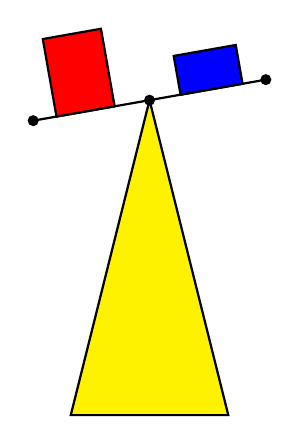
\begin{tikzpicture}[thick]
  \draw[fill=yellow] (0,0) -- (0:2) -- (1,4) coordinate (A) -- cycle;
  \fill[radius=2pt] (A) circle
    +(10:-1.5) circle coordinate (B)
    +(10:1.5) circle coordinate (C);
  \draw[black] (B) -- (C) coordinate[pos=0.1] (L) coordinate[pos=0.9] (R);
  \draw[fill=red] (L) -- ++(10:0.75) -- ([turn]90:1) -- ([turn]90:0.75) -- cycle;
  \draw[fill=blue] (R) -- ++(10:-0.8) -- ([turn]270:0.5) -- ([turn]270:0.8) -- cycle;
\end{tikzpicture}
%% *** END OF EXAMPLE CODE ***

\end{document}
